% Options for packages loaded elsewhere
\PassOptionsToPackage{unicode}{hyperref}
\PassOptionsToPackage{hyphens}{url}
\PassOptionsToPackage{dvipsnames,svgnames,x11names}{xcolor}
%
\documentclass[
  letterpaper,
  DIV=11]{scrartcl}

\usepackage{amsmath,amssymb}
\usepackage{iftex}
\ifPDFTeX
  \usepackage[T1]{fontenc}
  \usepackage[utf8]{inputenc}
  \usepackage{textcomp} % provide euro and other symbols
\else % if luatex or xetex
  \usepackage{unicode-math}
  \defaultfontfeatures{Scale=MatchLowercase}
  \defaultfontfeatures[\rmfamily]{Ligatures=TeX,Scale=1}
\fi
\usepackage{lmodern}
\ifPDFTeX\else  
    % xetex/luatex font selection
\fi
% Use upquote if available, for straight quotes in verbatim environments
\IfFileExists{upquote.sty}{\usepackage{upquote}}{}
\IfFileExists{microtype.sty}{% use microtype if available
  \usepackage[]{microtype}
  \UseMicrotypeSet[protrusion]{basicmath} % disable protrusion for tt fonts
}{}
\makeatletter
\@ifundefined{KOMAClassName}{% if non-KOMA class
  \IfFileExists{parskip.sty}{%
    \usepackage{parskip}
  }{% else
    \setlength{\parindent}{0pt}
    \setlength{\parskip}{6pt plus 2pt minus 1pt}}
}{% if KOMA class
  \KOMAoptions{parskip=half}}
\makeatother
\usepackage{xcolor}
\setlength{\emergencystretch}{3em} % prevent overfull lines
\setcounter{secnumdepth}{-\maxdimen} % remove section numbering
% Make \paragraph and \subparagraph free-standing
\ifx\paragraph\undefined\else
  \let\oldparagraph\paragraph
  \renewcommand{\paragraph}[1]{\oldparagraph{#1}\mbox{}}
\fi
\ifx\subparagraph\undefined\else
  \let\oldsubparagraph\subparagraph
  \renewcommand{\subparagraph}[1]{\oldsubparagraph{#1}\mbox{}}
\fi

\usepackage{color}
\usepackage{fancyvrb}
\newcommand{\VerbBar}{|}
\newcommand{\VERB}{\Verb[commandchars=\\\{\}]}
\DefineVerbatimEnvironment{Highlighting}{Verbatim}{commandchars=\\\{\}}
% Add ',fontsize=\small' for more characters per line
\usepackage{framed}
\definecolor{shadecolor}{RGB}{241,243,245}
\newenvironment{Shaded}{\begin{snugshade}}{\end{snugshade}}
\newcommand{\AlertTok}[1]{\textcolor[rgb]{0.68,0.00,0.00}{#1}}
\newcommand{\AnnotationTok}[1]{\textcolor[rgb]{0.37,0.37,0.37}{#1}}
\newcommand{\AttributeTok}[1]{\textcolor[rgb]{0.40,0.45,0.13}{#1}}
\newcommand{\BaseNTok}[1]{\textcolor[rgb]{0.68,0.00,0.00}{#1}}
\newcommand{\BuiltInTok}[1]{\textcolor[rgb]{0.00,0.23,0.31}{#1}}
\newcommand{\CharTok}[1]{\textcolor[rgb]{0.13,0.47,0.30}{#1}}
\newcommand{\CommentTok}[1]{\textcolor[rgb]{0.37,0.37,0.37}{#1}}
\newcommand{\CommentVarTok}[1]{\textcolor[rgb]{0.37,0.37,0.37}{\textit{#1}}}
\newcommand{\ConstantTok}[1]{\textcolor[rgb]{0.56,0.35,0.01}{#1}}
\newcommand{\ControlFlowTok}[1]{\textcolor[rgb]{0.00,0.23,0.31}{#1}}
\newcommand{\DataTypeTok}[1]{\textcolor[rgb]{0.68,0.00,0.00}{#1}}
\newcommand{\DecValTok}[1]{\textcolor[rgb]{0.68,0.00,0.00}{#1}}
\newcommand{\DocumentationTok}[1]{\textcolor[rgb]{0.37,0.37,0.37}{\textit{#1}}}
\newcommand{\ErrorTok}[1]{\textcolor[rgb]{0.68,0.00,0.00}{#1}}
\newcommand{\ExtensionTok}[1]{\textcolor[rgb]{0.00,0.23,0.31}{#1}}
\newcommand{\FloatTok}[1]{\textcolor[rgb]{0.68,0.00,0.00}{#1}}
\newcommand{\FunctionTok}[1]{\textcolor[rgb]{0.28,0.35,0.67}{#1}}
\newcommand{\ImportTok}[1]{\textcolor[rgb]{0.00,0.46,0.62}{#1}}
\newcommand{\InformationTok}[1]{\textcolor[rgb]{0.37,0.37,0.37}{#1}}
\newcommand{\KeywordTok}[1]{\textcolor[rgb]{0.00,0.23,0.31}{#1}}
\newcommand{\NormalTok}[1]{\textcolor[rgb]{0.00,0.23,0.31}{#1}}
\newcommand{\OperatorTok}[1]{\textcolor[rgb]{0.37,0.37,0.37}{#1}}
\newcommand{\OtherTok}[1]{\textcolor[rgb]{0.00,0.23,0.31}{#1}}
\newcommand{\PreprocessorTok}[1]{\textcolor[rgb]{0.68,0.00,0.00}{#1}}
\newcommand{\RegionMarkerTok}[1]{\textcolor[rgb]{0.00,0.23,0.31}{#1}}
\newcommand{\SpecialCharTok}[1]{\textcolor[rgb]{0.37,0.37,0.37}{#1}}
\newcommand{\SpecialStringTok}[1]{\textcolor[rgb]{0.13,0.47,0.30}{#1}}
\newcommand{\StringTok}[1]{\textcolor[rgb]{0.13,0.47,0.30}{#1}}
\newcommand{\VariableTok}[1]{\textcolor[rgb]{0.07,0.07,0.07}{#1}}
\newcommand{\VerbatimStringTok}[1]{\textcolor[rgb]{0.13,0.47,0.30}{#1}}
\newcommand{\WarningTok}[1]{\textcolor[rgb]{0.37,0.37,0.37}{\textit{#1}}}

\providecommand{\tightlist}{%
  \setlength{\itemsep}{0pt}\setlength{\parskip}{0pt}}\usepackage{longtable,booktabs,array}
\usepackage{calc} % for calculating minipage widths
% Correct order of tables after \paragraph or \subparagraph
\usepackage{etoolbox}
\makeatletter
\patchcmd\longtable{\par}{\if@noskipsec\mbox{}\fi\par}{}{}
\makeatother
% Allow footnotes in longtable head/foot
\IfFileExists{footnotehyper.sty}{\usepackage{footnotehyper}}{\usepackage{footnote}}
\makesavenoteenv{longtable}
\usepackage{graphicx}
\makeatletter
\def\maxwidth{\ifdim\Gin@nat@width>\linewidth\linewidth\else\Gin@nat@width\fi}
\def\maxheight{\ifdim\Gin@nat@height>\textheight\textheight\else\Gin@nat@height\fi}
\makeatother
% Scale images if necessary, so that they will not overflow the page
% margins by default, and it is still possible to overwrite the defaults
% using explicit options in \includegraphics[width, height, ...]{}
\setkeys{Gin}{width=\maxwidth,height=\maxheight,keepaspectratio}
% Set default figure placement to htbp
\makeatletter
\def\fps@figure{htbp}
\makeatother
\newlength{\cslhangindent}
\setlength{\cslhangindent}{1.5em}
\newlength{\csllabelwidth}
\setlength{\csllabelwidth}{3em}
\newlength{\cslentryspacingunit} % times entry-spacing
\setlength{\cslentryspacingunit}{\parskip}
\newenvironment{CSLReferences}[2] % #1 hanging-ident, #2 entry spacing
 {% don't indent paragraphs
  \setlength{\parindent}{0pt}
  % turn on hanging indent if param 1 is 1
  \ifodd #1
  \let\oldpar\par
  \def\par{\hangindent=\cslhangindent\oldpar}
  \fi
  % set entry spacing
  \setlength{\parskip}{#2\cslentryspacingunit}
 }%
 {}
\usepackage{calc}
\newcommand{\CSLBlock}[1]{#1\hfill\break}
\newcommand{\CSLLeftMargin}[1]{\parbox[t]{\csllabelwidth}{#1}}
\newcommand{\CSLRightInline}[1]{\parbox[t]{\linewidth - \csllabelwidth}{#1}\break}
\newcommand{\CSLIndent}[1]{\hspace{\cslhangindent}#1}

\usepackage[font=small,format=plain,labelfont=bf, labelsep=period,justification=justified,singlelinecheck=false]{caption}
\setcounter{section}{1}
\KOMAoption{captions}{tableheading}
\makeatletter
\makeatother
\makeatletter
\makeatother
\makeatletter
\@ifpackageloaded{caption}{}{\usepackage{caption}}
\AtBeginDocument{%
\ifdefined\contentsname
  \renewcommand*\contentsname{Inhaltsverzeichnis}
\else
  \newcommand\contentsname{Inhaltsverzeichnis}
\fi
\ifdefined\listfigurename
  \renewcommand*\listfigurename{Abbildungsverzeichnis}
\else
  \newcommand\listfigurename{Abbildungsverzeichnis}
\fi
\ifdefined\listtablename
  \renewcommand*\listtablename{Tabellenverzeichnis}
\else
  \newcommand\listtablename{Tabellenverzeichnis}
\fi
\ifdefined\figurename
  \renewcommand*\figurename{Abbildung}
\else
  \newcommand\figurename{Abbildung}
\fi
\ifdefined\tablename
  \renewcommand*\tablename{Tabelle}
\else
  \newcommand\tablename{Tabelle}
\fi
}
\@ifpackageloaded{float}{}{\usepackage{float}}
\floatstyle{ruled}
\@ifundefined{c@chapter}{\newfloat{codelisting}{h}{lop}}{\newfloat{codelisting}{h}{lop}[chapter]}
\floatname{codelisting}{Listing}
\newcommand*\listoflistings{\listof{codelisting}{Listingverzeichnis}}
\usepackage{amsthm}
\theoremstyle{plain}
\newtheorem{theorem}{Theorem}[section]
\theoremstyle{definition}
\newtheorem{definition}{Definition}[section]
\theoremstyle{remark}
\AtBeginDocument{\renewcommand*{\proofname}{Beweis}}
\newtheorem*{remark}{Anmerkung}
\newtheorem*{solution}{Lösung}
\makeatother
\makeatletter
\@ifpackageloaded{caption}{}{\usepackage{caption}}
\@ifpackageloaded{subcaption}{}{\usepackage{subcaption}}
\makeatother
\makeatletter
\@ifpackageloaded{tcolorbox}{}{\usepackage[skins,breakable]{tcolorbox}}
\makeatother
\makeatletter
\@ifundefined{shadecolor}{\definecolor{shadecolor}{rgb}{.97, .97, .97}}
\makeatother
\makeatletter
\makeatother
\makeatletter
\makeatother
\ifLuaTeX
\usepackage[bidi=basic]{babel}
\else
\usepackage[bidi=default]{babel}
\fi
\babelprovide[main,import]{ngerman}
% get rid of language-specific shorthands (see #6817):
\let\LanguageShortHands\languageshorthands
\def\languageshorthands#1{}
\ifLuaTeX
  \usepackage{selnolig}  % disable illegal ligatures
\fi
\IfFileExists{bookmark.sty}{\usepackage{bookmark}}{\usepackage{hyperref}}
\IfFileExists{xurl.sty}{\usepackage{xurl}}{} % add URL line breaks if available
\urlstyle{same} % disable monospaced font for URLs
\hypersetup{
  pdftitle={Regression},
  pdfauthor={Dirk Ostwald},
  pdflang={de},
  colorlinks=true,
  linkcolor={blue},
  filecolor={Maroon},
  citecolor={Blue},
  urlcolor={Blue},
  pdfcreator={LaTeX via pandoc}}

\title{Regression}
\author{Dirk Ostwald}
\date{2023-06-02}

\begin{document}
\maketitle
\ifdefined\Shaded\renewenvironment{Shaded}{\begin{tcolorbox}[sharp corners, boxrule=0pt, frame hidden, enhanced, breakable, interior hidden, borderline west={3pt}{0pt}{shadecolor}]}{\end{tcolorbox}}\fi

Fundamentales Ziel von Regressionsanalysen ist es, Beziehungen zwischen
unabhängigen und abhängigen Variablen zu modellieren. Ein zentrales
Thema dabei ist die Anpassung von Funktionen an beobachtete Datensätze.
Mit dem Begriff der \emph{Ausgleichsgerade} im Rahmen der \emph{Methode
der kleinsten Quadrate} und dem Begriff der \emph{einfachen linearen
Regression} wollen wir uns in diesem Abschnitt diesen zentralen Themen
der probabilistischen Datenmodellierung schrittweise nähern. Dabei
unterscheiden sich die Konzepte von Ausgleichsgerade und einfacher
lineare Regression in einem zentralem Aspekt: bei der Ausgleichsgerade
werden unabhängige und abhängige Variable nicht als Zufallsvariablen
modelliert, im Rahmen der einfachen linearen Regression nimmt die
abhängige Variable dann die Form einer Zufallsvariablen an. Im Kontext
der Korrelation schließlich werden sowohl abhängige als auch unabhängige
Variable als Zufallsvariablen modelliert.

Um die Konzepte dieses Abschnittes zu verdeutlichen, betrachten wir
einen Beispieldatensatz in dem die Anzahl an Psychotherapiestunden als
unabhängige Variable \(x\) der Symptomreduktion einer Gruppe von
\(n = 20\) Patient:innen als abhängige Variable \(y\) gegenüber gestellt
wird (Abbildung~\ref{fig-beispieldatensatz} ). Die visuelle Inspektion
dieses Datensatzes legt nahe, dass ein Mehr an Therapiestunden ein Mehr
an Symptomreduktion impliziert. Ziel der Methode der kleinsten Quadrate
und der einfachen linearen Regression ist es, diesen intuitiven
funktionalen Zusammenhang zwischen unabhängiger und abhängiger Variable
auf eine quantitative Basis zu stellen.

\begin{figure}

{\centering 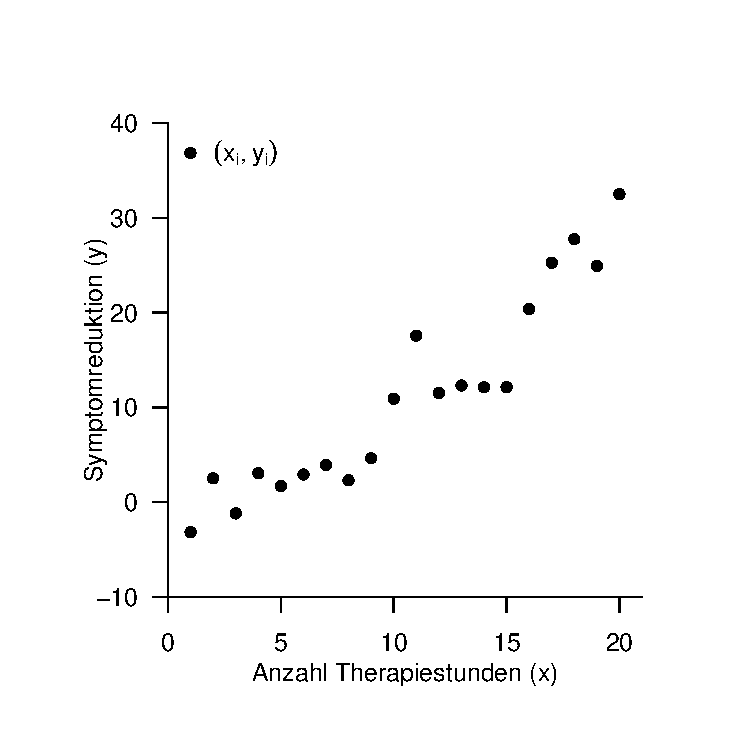
\includegraphics[width=0.5\textwidth,height=\textheight]{./Abbildungen/reg_beispieldatensatz.pdf}

}

\caption{\label{fig-beispieldatensatz}Beispieldatensatz}

\end{figure}

\hypertarget{sec-kq-methode}{%
\subsection{Methode der kleinsten Quadrate}\label{sec-kq-methode}}

Wir definieren zunächst den Begriff der \emph{Ausgleichsgerade}.

\begin{definition}[Ausgleichsgerade]\protect\hypertarget{def-ausgleichsgerade}{}\label{def-ausgleichsgerade}

Für \(\beta := (\beta_0,\beta_1)^T \in \mathbb{R}^2\) heißt die
linear-affine Funktion \begin{equation}
f_\beta : \mathbb{R} \to \mathbb{R}, x \mapsto f_\beta(x) := \beta_0 + \beta_1 x,
\end{equation} für die für einen Datensatz
\(\{(x_1,y_1),...,(x_n,y_n)\} \subset \mathbb{R}^2\) die Funktion
\begin{equation}
q : \mathbb{R}^2 \to \mathbb{R}_{\ge 0}, \beta \mapsto q(\beta)
:= \sum_{i=1}^n (y_i-f_\beta(x_i))^2
 = \sum_{i=1}^n (y_i- (\beta_0 + \beta_1x_i))^2
\end{equation} der quadrierten vertikalen Abweichungen der \(y_i\) von
den Funktionswerten \(f_{\beta}(x_i)\) ihr Minimum annimt,
\emph{Ausgleichsgerade für den Datensatz
\(\{(x_1,y_1),...,(x_n,y_n)\}\)}.

\end{definition}

Bei der Ausgleichsgerade handelt es sich also um eine
\emph{linear-affine Funktion} der Form \begin{equation}
f_\beta : \mathbb{R} \to \mathbb{R}, x \mapsto f_\beta(x) := \beta_0 + \beta_1 x.
\end{equation} Abbildung~\ref{fig-linear-affine-funktionen} zeigt drei
durch jeweils andere Werte von \(\beta_0\) und \(\beta_1\)
parameterisierte linear-affine Funktionen zusammen mit der Wertemenge
des Beispieldatensatzes.

Wie bei allen linear-affinen Funktionen entspricht bei \(f_\beta\) der
Wert von \(\beta_0\) dem Wert, den \(f_\beta\) für \(x = 0\) annimmt,
\begin{equation}
f_\beta(0) = \beta_0 + \beta_1\cdot0 = \beta_0
\end{equation} und damit graphisch dem Schnittpunkt des Funktionsgraphen
mit der \(y\)-Achse. Da \(\beta_0\) damit dem Versatz (engl.
\emph{offset}) des Funktionsgraphen von \(y = 0\) an der Stelle
\(x = 0\) entspricht, nennt man \(\beta_0\) auch häufig den
\emph{Offsetparameter}. Analog entspricht wie bei allen linear-affinen
Funktionen der Wert von \(\beta_1\) dem Wert der Funktionswertdifferenz
pro Argumenteinheitsdifferenz. Beispielsweise gilt etwa für
\(\beta_0 = 5\) und \(\beta_1 = 0.5\), dass \begin{align}
\begin{split}
f_\beta(2) - f_\beta(1) & =  (5 + 0.5\cdot2)  - (5 + 0.5\cdot1) = 1 - 0.5 = 0.5 \\
f_\beta(9) - f_\beta(8) & =  (5 + 0.5\cdot 9) - (5 + 0.5\cdot8) = 9.5 - 8 = 0.5
\end{split}
\end{align} Für eine Argumentdifferenz von \(1\) ergibt sich also eine
Funktionswertdifferenz von \(0.5\). \(\beta_1\) enkodiert also die
Stärke der Änderung der Funktionswerte pro Argumentseinheitsdifferenz
und damit die Steigung (engl. \emph{slope}) des Graphen der
linear-affinen Funktion. Entsprechend wird \(\beta_1\)
\emph{Steigungsparameter} oder \emph{Slopeparameter} genannt.

\begin{figure}

{\centering 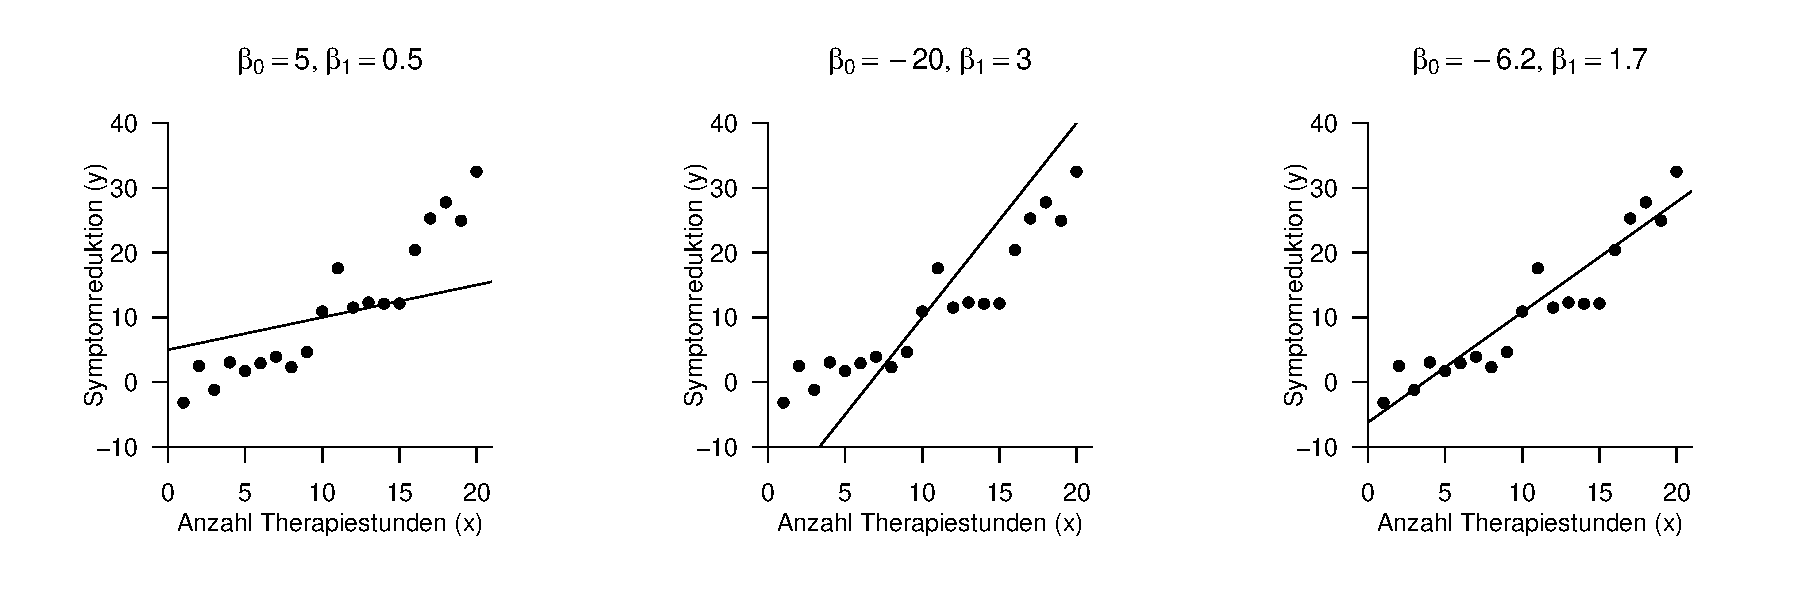
\includegraphics[width=1\textwidth,height=\textheight]{./Abbildungen/reg_linear_affine_funktionen.pdf}

}

\caption{\label{fig-linear-affine-funktionen}Linear-affine Funktionen
mit unterschiedlichen Parameterwerten vor dem Hintegrund des
Beispieldatensatzes}

\end{figure}

Nach Definition ist die Ausgleichsgerade nun allerdings nicht eine
beliebige linear-affine Funktion der Form \(f_\beta\), sondern eben
jene, die für einen gegebenen Datensatze \(\{(x_1,y_1),...,(x_n,y_n)\}\)
die Summe der quadrierten vertikalen Abweichnungen \begin{equation}
q(\beta) := \sum_{i=1}^n (y_i- (\beta_0 + \beta_1x_i))^2
\end{equation} minimiert. Für eine fest vorgegebenen Datensatz von
\((x_i,y_i)\) Paaren ist der Wert dieser Summe abhängig von den Werten
von \(\beta_0\) und \(\beta_1\) und kann deshalb durch Wahl geeigneter
Werte von \(\beta_0\) und \(\beta_1\) minimiert werden. Da hierbei eine
Summe von quadrierten Abweichungen zwischen Datenpunkten und Werten der
Ausgleichsgerade minimiert wird, spricht man auch oft etwas ungenau von
der \emph{Methode der kleinsten Quadrate} (engl. \emph{method of least
squares}). Abbildung~\ref{fig-vertikale-Abweichungen} zeigt die
vertikalen Abweichungen zwischen \(y_i\) und \(\beta_0 + \beta_1x_i\)
für \(i = 1,...,n\) des Beispieldatensatzes als orange Linien sowie die
Summe ihrer Quadrate \(q(\beta)\) im Titel. Für die Parameterwerte
\(\beta_0 = -6.2\) und \(\beta_1 = 1.7\) (vgl.
Abbildung~\ref{fig-linear-affine-funktionen}) nimmt diese Summe ihren
kleinsten Wert an.

\begin{figure}

{\centering 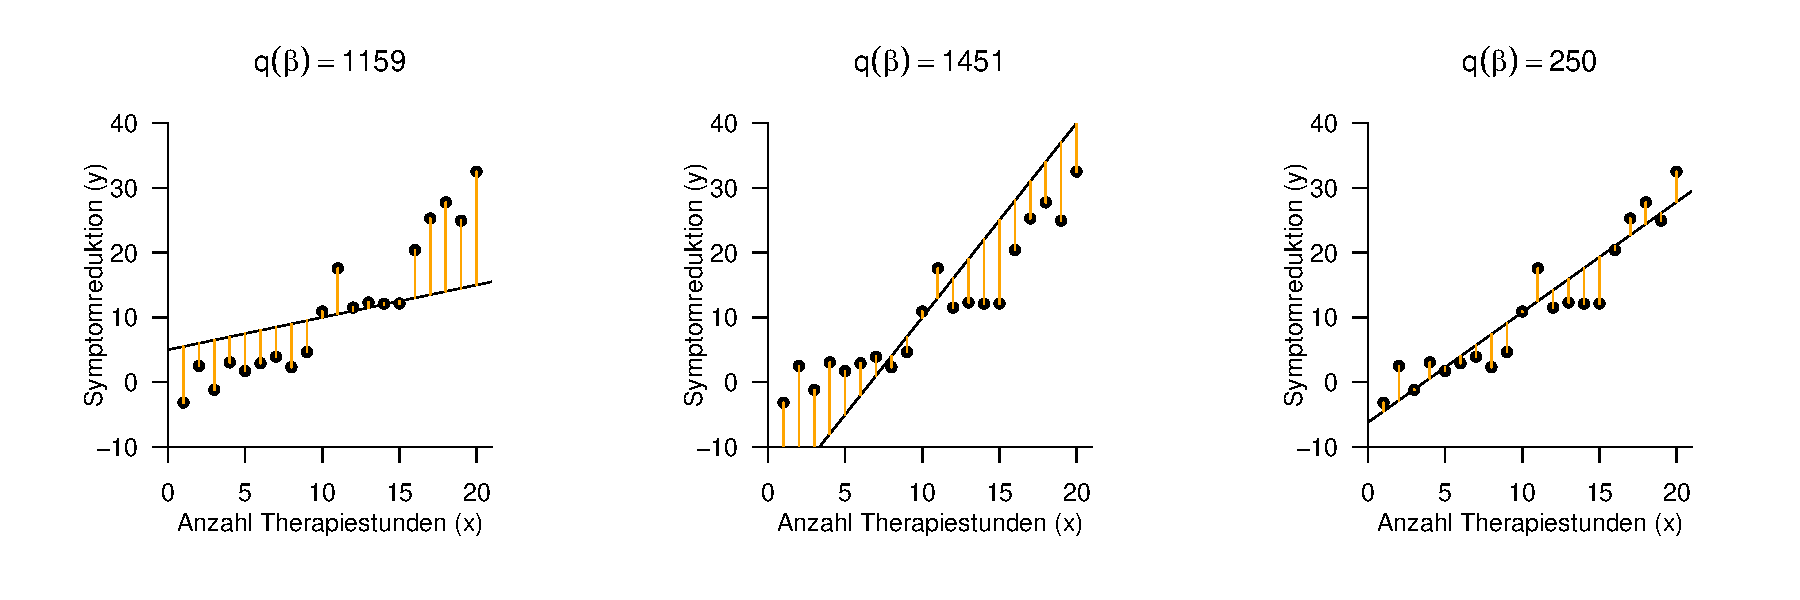
\includegraphics[width=1\textwidth,height=\textheight]{./Abbildungen/reg_vertikale_Abweichungen.pdf}

}

\caption{\label{fig-vertikale-Abweichungen}Vertikale Abweichungen und
Quadratsummen bei unterschiedlichen Parameterwerten}

\end{figure}

Konkrete Formeln zur Bestimmung der Parameterwerte der Ausgleichsgerade
stellt Theorem~\ref{thm-ausgleichsgerade} bereit.

\begin{theorem}[Ausgleichsgerade]\protect\hypertarget{thm-ausgleichsgerade}{}\label{thm-ausgleichsgerade}

Für einen Datensatz \(\{(x_1,y_1),...,(x_n,y_n)\}\subset\mathbb{R}^2\)
hat die Ausgleichsgerade die Form \begin{equation}
f_\beta : \mathbb{R} \to \mathbb{R}, x \mapsto f_\beta(x) := \hat{\beta}_0 + \hat{\beta}_1 x,
\end{equation} wobei mit der Stichprobenkovarianz \(c_{xy}\) der
\((x_i,y_i)\)-Werte, der Stichprobenvarianz \(s_x^2\) der \(x_i\)-Werte
und den Stichprobenmitteln \(\bar{x}\) und \(\bar{y}\) der \(x_i\)- und
\(y_i\)-Werte, respektive, gilt, dass \begin{equation}
\hat{\beta}_1 = \frac{c_{xy}}{s_x^2} \mbox{ und } \hat{\beta}_0 = \bar{y} - \hat{\beta}_1\bar{x}.
\end{equation}

\end{theorem}

\begin{proof}

\end{proof}

Theorem~\ref{thm-ausgleichsgerade} besagt, dass die Parameterwerte, die
für einen gegebenen Datensatz \(\{(x_1,y_1),...,(x_n,y_n)\}\) die Summe
der quadrierten vertikalen Abweichungen für eine linear-affine Funktion
minimieren mithilfe der Stichprobenmittel der \(x_i\)- und
\(y_i\)-Werte, der Stichprobenvarianz der \(x_i\)-Werte und der
Stichprobenkovarianz der \(x_i\)- und \(y_i\)-Werte berechnet werden
können. Die Terminologie orientiert sich hier an den Begrifflichkeiten
der deskriptiven Statistik, insbesondere werden die \(x_i\)-Werte häufig
\emph{nicht} als Realisationen von Zufallsvariablen verstanden, der
Begriff der Stichprobe wird jedoch trotzdem verwendet. Aus der
Anwendungsperspektive können nach Theorem~\ref{thm-ausgleichsgerade} die
Parameter der Ausgleichsgerade also mithilfe der bekannten Funktionen
für die Auswertung deskriptiver Statistiken bestimmt werden. Folgender
\textbf{R} Code demonstriert dies.

\tiny

\begin{Shaded}
\begin{Highlighting}[]
\CommentTok{\# Einlesen des Beispieldatensatzes}
\NormalTok{fname       }\OtherTok{=} \FunctionTok{file.path}\NormalTok{(}\StringTok{"./Daten/Regression.csv"}\NormalTok{)}
\NormalTok{D           }\OtherTok{=} \FunctionTok{read.table}\NormalTok{(fname, }\AttributeTok{sep =} \StringTok{","}\NormalTok{, }\AttributeTok{header =} \ConstantTok{TRUE}\NormalTok{)}

\CommentTok{\# Stichprobenstatistiken}
\NormalTok{x\_bar       }\OtherTok{=} \FunctionTok{mean}\NormalTok{(D}\SpecialCharTok{$}\NormalTok{x\_i)               }\CommentTok{\# Stichprobenmittel der x\_i{-}Werte}
\NormalTok{y\_bar       }\OtherTok{=} \FunctionTok{mean}\NormalTok{(D}\SpecialCharTok{$}\NormalTok{y\_i)               }\CommentTok{\# Stichprobenmittel der y\_i{-}Werte}
\NormalTok{s2x         }\OtherTok{=} \FunctionTok{var}\NormalTok{(D}\SpecialCharTok{$}\NormalTok{x\_i)                }\CommentTok{\# Stichprobenvarianz der  x\_i{-}Werte}
\NormalTok{cxy         }\OtherTok{=} \FunctionTok{cov}\NormalTok{(D}\SpecialCharTok{$}\NormalTok{x\_i, D}\SpecialCharTok{$}\NormalTok{y\_i)         }\CommentTok{\# Stichprobenkovarianz der (x\_i,y\_i){-}Werte}

\CommentTok{\# Ausgleichsgeradenparameter}
\NormalTok{beta\_1\_hat  }\OtherTok{=}\NormalTok{ cxy}\SpecialCharTok{/}\NormalTok{s2x                   }\CommentTok{\# \textbackslash{}hat\{\textbackslash{}beta\}\_1, Steigungsparameter}
\NormalTok{beta\_0\_hat  }\OtherTok{=}\NormalTok{ y\_bar }\SpecialCharTok{{-}}\NormalTok{ beta\_1\_hat}\SpecialCharTok{*}\NormalTok{x\_bar  }\CommentTok{\# \textbackslash{}hat\{\textbackslash{}beta\}\_0, Offset Parameter}

\CommentTok{\# Ausgabe}
\FunctionTok{cat}\NormalTok{(}\StringTok{"beta\_0\_hat:"}\NormalTok{, beta\_0\_hat,}
    \StringTok{"}\SpecialCharTok{\textbackslash{}n}\StringTok{beta\_1\_hat:"}\NormalTok{, beta\_1\_hat)}
\end{Highlighting}
\end{Shaded}

\begin{verbatim}
beta_0_hat: -6.194704 
beta_1_hat: 1.657055
\end{verbatim}

\normalsize

Eine typische Visualisierung der Ausgleichsgerade eines Datensatzes wie
in Abbildung~\ref{fig-ausgleichsgerade} implementiert folgender
\textbf{R} Code.

\tiny

\begin{Shaded}
\begin{Highlighting}[]
\CommentTok{\# Visualisierung der Datenwerte als Punktwolke}
\FunctionTok{plot}\NormalTok{(}
\NormalTok{D}\SpecialCharTok{$}\NormalTok{x\_i,}
\NormalTok{D}\SpecialCharTok{$}\NormalTok{y\_i,}
\AttributeTok{pch         =} \DecValTok{16}\NormalTok{,}
\AttributeTok{xlab        =} \StringTok{"Anzahl Therapiestunden (x)"}\NormalTok{,}
\AttributeTok{ylab        =} \StringTok{"Symptomreduktion (y)"}\NormalTok{,}
\AttributeTok{xlim        =} \FunctionTok{c}\NormalTok{(}\DecValTok{0}\NormalTok{,}\DecValTok{21}\NormalTok{),}
\AttributeTok{ylim        =} \FunctionTok{c}\NormalTok{(}\SpecialCharTok{{-}}\DecValTok{10}\NormalTok{, }\DecValTok{40}\NormalTok{),}
\AttributeTok{main        =} \FunctionTok{TeX}\NormalTok{(}\StringTok{"$}\SpecialCharTok{\textbackslash{}\textbackslash{}}\StringTok{hat\{}\SpecialCharTok{\textbackslash{}\textbackslash{}}\StringTok{beta\}\_0 =  {-}6.19, }\SpecialCharTok{\textbackslash{}\textbackslash{}}\StringTok{hat\{}\SpecialCharTok{\textbackslash{}\textbackslash{}}\StringTok{beta\}\_1 = 1.66$"}\NormalTok{))}

\CommentTok{\# Ausgleichsgerade}
\FunctionTok{abline}\NormalTok{(}
\AttributeTok{coef        =} \FunctionTok{c}\NormalTok{(beta\_0\_hat, beta\_1\_hat),}
\AttributeTok{lty         =} \DecValTok{1}\NormalTok{,}
\AttributeTok{col         =} \StringTok{"black"}\NormalTok{)}

\CommentTok{\# Legende}
\FunctionTok{legend}\NormalTok{(}
\StringTok{"topleft"}\NormalTok{,}
\FunctionTok{c}\NormalTok{(}\FunctionTok{TeX}\NormalTok{(}\StringTok{"$(x\_i,y\_i)$"}\NormalTok{), }\FunctionTok{TeX}\NormalTok{(}\StringTok{"$f(x) = }\SpecialCharTok{\textbackslash{}\textbackslash{}}\StringTok{hat\{}\SpecialCharTok{\textbackslash{}\textbackslash{}}\StringTok{beta\}\_0 + }\SpecialCharTok{\textbackslash{}\textbackslash{}}\StringTok{hat\{}\SpecialCharTok{\textbackslash{}\textbackslash{}}\StringTok{beta\}\_1x$"}\NormalTok{)),}
\AttributeTok{lty        =} \FunctionTok{c}\NormalTok{(}\DecValTok{0}\NormalTok{,}\DecValTok{1}\NormalTok{),}
\AttributeTok{pch        =} \FunctionTok{c}\NormalTok{(}\DecValTok{16}\NormalTok{, }\ConstantTok{NA}\NormalTok{),}
\AttributeTok{bty        =} \StringTok{"n"}\NormalTok{)}
\end{Highlighting}
\end{Shaded}

\normalsize

\begin{figure}

{\centering 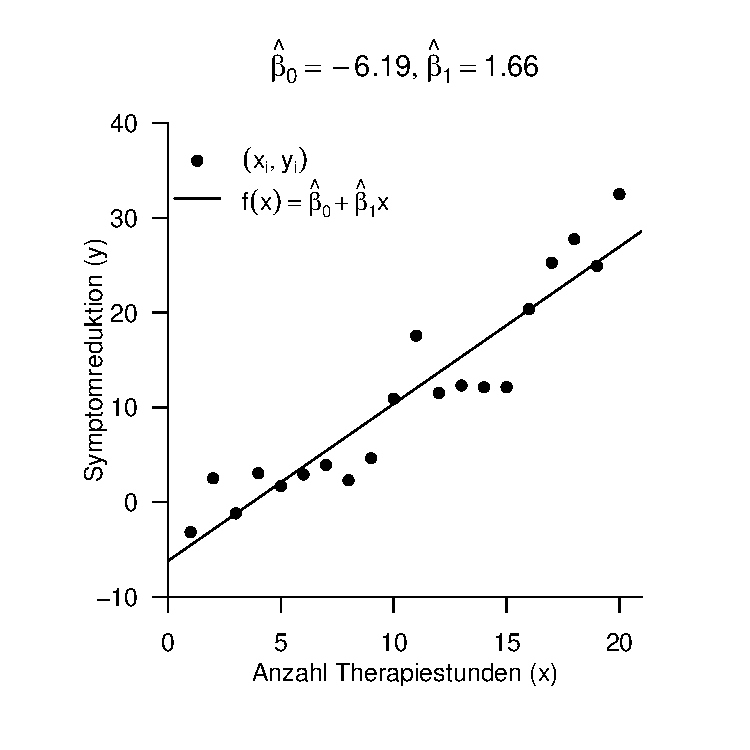
\includegraphics[width=0.5\textwidth,height=\textheight]{./Abbildungen/reg_ausgleichsgerade.pdf}

}

\caption{\label{fig-ausgleichsgerade}Ausgleichsgerade für den
Beispieldatensatz}

\end{figure}

\hypertarget{literaturhinweise}{%
\subsection{Literaturhinweise}\label{literaturhinweise}}

Die Idee der Minimierung einer Summe von quadrierten Abweichungen bei
der Anpassung einer Polynomfunktion an beobachtete Werte geht auf die
Arbeiten von Legendre (1805) und Gauss (1809) im Kontext der Bestimmung
von Planetenbahnen zurück. Eine historische Einordnung dazu gibt Stigler
(1981). Der Begriff der Regression geht zurück auf Galton (1886).
Stigler (1986) gibt dazu einen ausführlichen historischen Überblick.

\hypertarget{referenzen}{%
\subsection*{Referenzen}\label{referenzen}}
\addcontentsline{toc}{subsection}{Referenzen}

\hypertarget{refs}{}
\begin{CSLReferences}{1}{0}
\leavevmode\vadjust pre{\hypertarget{ref-galton1886}{}}%
Galton, Francis. 1886. {„Regression {Towards Mediocrity} in {Hereditary
Stature}.``} \emph{The Journal of the Anthropological Institute of Great
Britain and Ireland} 15: 246. \url{https://doi.org/10.2307/2841583}.

\leavevmode\vadjust pre{\hypertarget{ref-gauss1809}{}}%
Gauss, Carl Friedrich. 1809. \emph{Theoria {Motus Corporum Coelestium}
in {Sectionibus Conicis Solem Ambientium}}. {Cambridge}: {Cambridge
University Press}.

\leavevmode\vadjust pre{\hypertarget{ref-legendre1805}{}}%
Legendre, A. M. 1805. \emph{Nouvelles Methodes Pour La Determination Des
Orbites Des Cometes}. {Didot Paris}.

\leavevmode\vadjust pre{\hypertarget{ref-stigler1981}{}}%
Stigler, Stephen M. 1981. {„Gauss and the {Invention} of {Least
Squares}``}. \emph{The Annals of Statistics} 9 (3).
\url{https://doi.org/10.1214/aos/1176345451}.

\leavevmode\vadjust pre{\hypertarget{ref-stigler1986}{}}%
---------. 1986. \emph{The History of Statistics: The Measurement of
Uncertainty Before 1900}. {Cambridge, Mass}: {Belknap Press of Harvard
University Press}.

\end{CSLReferences}



\end{document}
